\documentclass[11pt]{article}
\usepackage[margin=1in]{geometry}
\usepackage{graphicx}
\usepackage{booktabs}
\usepackage{array}
\usepackage{fancyhdr}
\usepackage{enumitem}
\usepackage{hyperref}
\usepackage{tabularx}

\setlength{\parindent}{0pt}
\setlength{\parskip}{1\baselineskip}

\setlength{\headheight}{22.1pt}
\addtolength{\topmargin}{-0.1pt}
\pagestyle{fancy}
\fancyhf{}
\lhead{
\includegraphics[height=18pt]{noulogo.png}}
\rhead{TFM}
\cfoot{\thepage}
\renewcommand{\headrulewidth}{0.4pt}

\renewcommand{\contentsname}{Índice de Contenidos}
\renewcommand{\figurename}{Figura}
\renewcommand{\tablename}{Tabla}
\graphicspath{{images/}}

\begin{document}
	\pagenumbering{gobble}
	
	\begin{titlepage}
		\centering
		\vspace*{1cm}
		
\includegraphics[height=60pt]{noulogo.png}\par
		\vspace{1.5cm}
		{\LARGE \textbf{Identificación y modelización de una firma transcriptómica asociada a metástasis ganglionar mediante análisis pseudobulk de datos single-cell RNA-seq}\par}
		\vspace{1cm}
		{\Large Trabajo Fin de Máster \\ 
			Máster en Bioinformática y Bioestadística \\
			2026 \par}
		\vspace{1cm}
		{\large Francisco Manuel González Nuño}\par
		\vspace{0.2cm}
		{\large Tutora: Izaskun Mallona}\par
		\vspace{0.25cm}
		{\large Análisis de datos ómicos}\par
		\vfill
		% {\large Fecha}\par
	\end{titlepage}
	
	\tableofcontents
	\listoftables
	\listoffigures
	\pagenumbering{arabic}
	\newpage
	
	\section{Tabla resumen}
		\begin{tabular}{p{0.2\linewidth}p{0.75\linewidth}@{}}
			\toprule
			\textbf{Título provisional} & Identificación y modelización de una firma transcriptómica asociada a metástasis ganglionar mediante análisis pseudobulk de datos single-cell RNA-seq. \\
			
			\textbf{Palabras clave} & scRNA-seq; tumor heterogeneity; colorectal cancer; transcriptomics; pseudobulk analysis; machine learning; artificial intelligence\\
			\bottomrule
		\end{tabular}
	
	\section{Contexto y justificación del trabajo}
		El cáncer colorrectal (CRC) constituye uno de los tumores con mayor incidencia y mortalidad a nivel mundial. Según el informe GLOBOCAN\footnotemark 2020, el CRC representa el tercer cáncer más diagnosticado y la segunda causa de muerte por cáncer a nivel global [\ref{bib:globocan}]. A pesar de los avances terapéuticos, la progresión metastásica continúa siendo el principal determinante del pronóstico.
		
		\footnotetext{\url{https://gco.iarc.fr/en}}
		
		Un elemento clave en la progresión tumoral es la heterogeneidad intratumoral, entendida como la coexistencia de subpoblaciones celulares molecularmente distintas dentro de un mismo tumor. Esta heterogeneidad influye en la evolución clonal, la adaptación al microambiente y la resistencia a tratamientos [\ref{bib:tumor_hetereogeneity}].
		
		Las aproximaciones transcriptómicas bulk tradicionales proporcionan una señal promedio de la muestra, lo que dificulta la detección de subclones minoritarios o estados celulares transitorios. La aparición de la transcriptómica de célula única (single-cell RNA sequencing, scRNA-seq) ha permitido superar esta limitación, ofreciendo una resolución sin precedentes en la caracterización de la variabilidad celular [\ref{bib:RNA_seq_trad_1}, \ref{bib:RNA_seq_trad_2}].
		
		El conjunto de datos público \textit{GSE97693}, publicado en \textit{Science} [\ref{bib:PAPER}], constituye un recurso relevante para estudiar la heterogeneidad tumoral en cáncer colorrectal mediante \textit{scTrio-seq2}, técnica que permite analizar simultáneamente transcriptómica y metilación a nivel de célula individual. Este tipo de datos proporciona un escenario idóneo para aplicar técnicas computacionales avanzadas.
		
		El análisis de datos de célula única presenta retos metodológicos específicos, tales como la alta dimensionalidad, la dispersión de los datos, el ruido técnico y la variabilidad interpaciente. En este escenario, las técnicas de inteligencia artificial, como el aprendizaje automático (\textit{machine learning}), se han consolidado como herramientas esenciales para la reducción de dimensionalidad, la integración de datos y la eliminación de efectos de lote (\textit{batch effect}), permitiendo una caracterización robusta de los estados celulares [\ref{bib:tutorial}].
		
		
		
		
		El presente trabajo se justifica mediante distintos aspectos clave. En primer lugar, la importancia clínica y epidemiológica del cáncer colorrectal, que continúa siendo uno de los principales retos en salud pública. En segundo lugar, la necesidad de disponer de metodologías avanzadas capaces de caracterizar la heterogeneidad tumoral, un fenómeno central en la progresión del cáncer y en la respuesta terapéutica. Asimismo, este trabajo aprovecha la oportunidad de aplicar técnicas de \textit{machine learning} a datos reales de \textit{single-cell}, un ámbito en rápida expansión que permite explorar la complejidad celular con una resolución sin precedentes. 
				
		
		En conjunto, este trabajo aborda un problema biomédico de relevancia mediante herramientas computacionales avanzadas y un enfoque metodológico riguroso.

	
	\section{Descripción general}
	
		Este Trabajo Fin de Máster se centrará en el estudio de la heterogeneidad transcriptómica del cáncer colorrectal a resolución de célula individual, con especial énfasis en la identificación de programas moleculares asociados a la progresión metastásica. A partir de datos de secuenciación de ARN de célula única procedentes de tumor primario, metástasis ganglionar y tejido normal adyacente, el proyecto abordará el análisis integrado de la arquitectura celular tumoral y los cambios transcriptómicos vinculados a la diseminación tumoral.
		
		
		El eje central del trabajo será la exploración y caracterización de una posible firma transcriptómica asociada a la progresión metastásica, entendida como un conjunto coherente de genes cuya expresión distingue las células tumorales del tumor primario de aquellas presentes en metástasis ganglionar. La firma se analizará integrada en la arquitectura celular del tumor, atendiendo tanto a la variedad de estados celulares presentes como a la contribución relativa de los distintos tipos celulares al fenotipo metastásico. 
		
		
		El trabajo se estructurará en varias fases. En primer lugar, se realizará un análisis exploratorio y reducción de dimensionalidad mediante técnicas como PCA o UMAP. Seguidamente, se analizarán las posibles subpoblaciones celulares que serán anotadas mediante métodos automáticos de referencia.
		
		
		En una segunda fase, el análisis se centrará en comparar las células de las distintas regiones (tejido normal, tumor primario y metástasis ganglionar) con el fin de identificar diferencias transcriptómicas asociadas a la progresión tumoral. Se emplearán enfoques de análisis diferencial junto con técnicas de análisis y modelos de aprendizaje automático para identificar los genes con mayor capacidad discriminativa entre ambas localizaciones.
		
		
		Finalmente, se evaluará de manera exploratoria la asociación entre la activación de la firma metastásica, la composición celular tumoral y variables clínicas como el estadio AJCC, con el fin de explorar posibles relaciones entre heterogeneidad transcriptómica y progresión clínica.
		
		
		En conjunto, el proyecto combinará análisis de heterogeneidad celular, estadística inferencial y técnicas de aprendizaje automático interpretables para caracterizar los programas moleculares asociados a la metástasis en cáncer colorrectal, integrando información biológica y clínica dentro de un marco metodológico coherente.
		
		
	\section{Objetivos del proyecto}
		
		\subsection{Objetivo general}
			Identificar y caracterizar una posible firma transcriptómica asociada al desarrollo tumoral en cáncer colorrectal mediante el análisis de datos de secuenciación de ARN a nivel de célula individual, integrando el estudio de la heterogeneidad celular tumoral, la modelización computacional y el contexto clínico disponible.
			
		\subsection{Objetivos específicos}
			\begin{enumerate}
				\item Reconstruir la arquitectura celular del cáncer colorrectal a resolución single-cell, identificando subpoblaciones y estados celulares relevantes, con especial atención al compartimento epitelial tumoral.
				
				\item Identificar un potencial conjunto de genes diferencialmente expresados entre células de tumor primario y metástasis ganglionar.
				
				\item Evaluar la capacidad discriminativa de la firma metastásica mediante modelos supervisados de aprendizaje automático interpretables, identificando posibles variables génicas con mayor contribución al modelo discriminante.
				
				\item Analizar la relevancia funcional y biológica de los genes identificados asociados a la metástasis mediante análisis de enriquecimiento y contextualización en procesos implicados en progresión tumoral.
				
				\item Realizar un análisis integrado de actividad de vías y reguladores en scRNA‑seq.
				
				\item Implementar el análisis en un entorno computacional estructurado que garantice la trazabilidad y reproducibilidad de los resultados.
			\end{enumerate}
		
		\subsection{Objetivos secundarios complementarios}
			\begin{enumerate}
				\item Comparar de manera exploratoria la activación de la firma metastásica con el tejido normal adyacente, evaluando posibles gradientes transcriptómicos entre tejido normal, tumor primario y metástasis ganglionar.
				
				\item Analizar posibles diferencias en la composición celular entre tumor primario y metástasis ganglionar y su contribución al fenotipo metastásico.
				
				\item Explorar la asociación entre la intensidad de activación de la firma metastásica y variables clínicas disponibles, como el estadio tumoral (AJCC).
				
				\item Evaluar la robustez de la firma identificada mediante estrategias adicionales de validación interna (por ejemplo, esquemas de validación leave-one-out).
			\end{enumerate}
		
		
	\section{Enfoque y método a seguir}
		
		El estudio de la progresión metastásica en cáncer colorrectal a partir de datos transcriptómicos puede abordarse mediante distintas estrategias analíticas, que difieren tanto en el nivel de resolución considerado como en el marco estadístico empleado.
		
		\subsection{Estrategias posibles consideradas}
			
			Una primera estrategia consistiría en realizar un análisis transcriptómico convencional a nivel de muestra agregada, utilizando perfiles promedio o pseudobulk sin considerar explícitamente la heterogeneidad celular. Este enfoque simplifica la dimensionalidad del problema y permite aplicar metodologías estadísticas bien establecidas, pero pierde la resolución celular que caracteriza a los datos single-cell y puede enmascarar estados celulares minoritarios relevantes para la progresión metastásica.
			
			Una segunda estrategia sería plantear el análisis exclusivamente a nivel celular, comparando directamente células individuales del tumor primario y de la metástasis ganglionar. Este enfoque explota plenamente la resolución single-cell, pero introduce dependencias estadísticas entre células del mismo paciente y puede sobreestimar la potencia si no se controla adecuadamente la variabilidad interpaciente.
			
			Una tercera estrategia, más integradora, combina ambos niveles: utiliza el análisis single-cell para reconstruir la arquitectura celular y definir subpoblaciones relevantes, y posteriormente aplica estrategias de agregación controlada (pseudobulk por paciente y tejido) para realizar comparaciones diferenciales y desarrollar modelos supervisados minimizando la dependencia entre observaciones.
			
		\subsection{Estrategia elegida}
			
			En este trabajo se optará por una estrategia integradora que permitirá explotar la riqueza informativa de los datos single-cell sin ignorar la estructura jerárquica del diseño experimental.
			
			\paragraph{Justificación:} 
			
			La estrategia seleccionada se considera la más adecuada por varias razones. En primer lugar, permite preservar la resolución celular necesaria para estudiar la heterogeneidad tumoral, elemento central del proyecto. En segundo lugar, el uso de agregación por paciente reduce el riesgo de pseudorreplicación y mejora la validez estadística de las comparaciones entre tumor primario y metástasis ganglionar. En tercer lugar, la incorporación de modelos supervisados interpretables facilita la identificación de genes con capacidad discriminativa real, más allá de diferencias estadísticas aisladas.
			
			Asimismo, este enfoque permite integrar análisis exploratorios adicionales, como la comparación con tejido normal o la asociación con variables clínicas, sin comprometer la coherencia del núcleo metodológico.
			
			En conjunto, la estrategia adoptada equilibra resolución biológica, rigor estadístico e interpretabilidad computacional, alineándose de forma directa con los objetivos planteados en el proyecto.
			
	\section{Impacto en sostenibilidad, ético-social y de diversidad}
		
		El proyecto impacta principalmente en la categoría \textit{ODS 3 - Salud y bienestar}, promovido por Naciones Unidas\footnotemark, al contribuir al avance en la comprensión molecular de la progresión metastásica en cáncer colorrectal, una de las principales causas de mortalidad oncológica a nivel global.
		
		\footnotetext{\url{https://www.un.org/sustainabledevelopment/es/sustainable-development-goals/}}
		
		Desde una perspectiva ético-social, el trabajo se fundamenta exclusivamente en el análisis de datos públicos previamente anonimizados y con aprobación ética, sin implicar intervención directa sobre pacientess. Esto garantiza el respeto a los principios de confidencialidad, no maleficencia y uso responsable de la información biomédica.
		
		Asimismo, el conjunto de datos utilizado incluye muestras procedentes tanto de hombres como de mujeres, permitiendo un análisis que contempla la diversidad biológica y evita sesgos derivados de estudios centrados en un único sexo.
		
		Desde el punto de vista de sostenibilidad ecológica, el proyecto presenta un impacto ambiental reducido al basarse exclusivamente en datos ya generados, evitando el consumo de reactivos o recursos experimentales.
		
%		Finalmente, el desarrollo de un pipeline reproducible favorece la transparencia científica y reduce la duplicación innecesaria de esfuerzos en investigación futura, promoviendo una ciencia más sostenible y colaborativa.
		
		
		
	\section{Planificación}
		\subsection{Tareas}
		
		\begin{enumerate}
			\item Preparación e integración de los datos.
				\subitem Recopilación y organización de archivos TPM individuales.
				\subitem Construcción de la matriz de expresión consolidada.
				\subitem Integración de metadatos (paciente, tejido, estadio, localización anatómica).
				\subitem Verificación de correspondencia entre expresión y metadatos.
				\subitem Exploración inicial de dimensiones y estructura del dataset.
				
			\item Caracterización de la arquitectura celular.
				\subitem Reducción de dimensionalidad (PCA).
				\subitem Construcción de representación no lineal (UMAP).
				\subitem Clustering no supervisado.
				\subitem Identificación de marcadores por cluster.
				\subitem Anotación celular mediante métodos automáticos y marcadores conocidos.
				\subitem Evaluación de estabilidad del clustering.
				
			\item Análisis composicional.
				\subitem Cálculo de proporciones celulares por paciente y tejido.
				\subitem Comparación exploratoria entre tumor primario y metástasis.
				\subitem Visualización de cambios composicionales.
				
			\item Identificación de la firma metastásica.
				\subitem Selección de células epiteliales tumorales.
				\subitem Generación de perfiles pseudobulk por paciente y localización.
				\subitem Análisis diferencial PT vs LN.
				\subitem Control de variabilidad interpaciente.
				\subitem Identificación preliminar de genes candidatos.
				
			\item Modelización.
				\subitem Selección de variables candidatas.
				\subitem División de datos para validación.
				\subitem Entrenamiento de modelos supervisados.
				\subitem Evaluación del rendimiento.
				\subitem Extracción de importancia de variables.
				\subitem Evaluación de estabilidad del modelo.
				
				
			\item Construcción de una puntuación metastásica.
				\subitem Definición del método de agregación de la firma.
				\subitem Cálculo del puntaje por célula.
				\subitem Agregación por paciente.
				\subitem Visualización de gradientes (normal, tumor primario, metástasis ganglionar).
				
				
			\item Análisis funcional y de actividad de vías y reguladores.
				\subitem Preparación de listas génicas.
				\subitem Análisis de enriquecimiento (GO, KEGG, Reactome).
				\subitem Análisis de actividad de vías y reguladores.
				\subitem Interpretación biológica de resultados.
				\subitem Integración con literatura científica.
				
			\item Análisis exploratorios adicionales.
				\subitem Comparación con tejido normal.
				\subitem Asociación exploratoria con estadio clínico.
				\subitem Análisis de robustez adicional.
				
			\item Redacción de la memoria final.
		\end{enumerate}
		
		\subsection{Calendario}
			
La planificación de tareas y subtareas se ha realizado reflejando aquellas identificadas como principales, cuya duración queda recogida en la tabla \ref{tab:calendario} y representada gráficamente en la figura \ref{fig:Gantt}.
			
			
			\begin{table}[h!]
				\centering
				\caption{Calendario y distribución de tareas.} \label{tab:calendario}
				\resizebox{\textwidth}{!}{
				\begin{tabular}{l l l l c}
					\hline
					\textbf{Nombre} & \textbf{Nivel} & \textbf{Inicio} & \textbf{Fin} & \textbf{Duración} \\
					\hline
					Preparación e integración de datos & TAREA & 04-mar & 09-mar & 5 \\
					Arquitectura celular & TAREA & 09-mar & 24-mar & 15 \\
					Reducción dimensional & SUBTAREA & 09-mar & 14-mar & 5 \\
					Clustering & SUBTAREA & 14-mar & 19-mar & 5 \\
					Anotación celular & SUBTAREA & 19-mar & 24-mar & 5 \\
					Análisis composicional & TAREA & 24-mar & 27-mar & 3 \\
					Identificación firma metastásica & TAREA & 27-mar & 18-abr & 22 \\
					Filtrado epitelial & SUBTAREA & 27-mar & 30-mar & 3 \\
					Generación pseudobulk & SUBTAREA & 30-mar & 04-abr & 5 \\
					Análisis diferencial PT vs LN & SUBTAREA & 04-abr & 11-abr & 7 \\
					Refinamiento firma & SUBTAREA & 11-abr & 18-abr & 7 \\
					Modelización supervisada & TAREA & 18-abr & 03-may & 15 \\
					Selección variables & SUBTAREA & 18-abr & 21-abr & 3 \\
					Entrenamiento ML & SUBTAREA & 21-abr & 28-abr & 7 \\
					Validación modelo & SUBTAREA & 28-abr & 03-may & 5 \\
					Construcción metastatic score & TAREA & 03-may & 08-may & 5 \\
					Análisis funcional & TAREA & 08-may & 13-may & 5 \\
					Análisis exploratorios & TAREA & 13-may & 19-may & 6 \\
					Redacción e integración final & TAREA & 05-mar & 03-jun & 90 \\
					Documento finalizado & HITO & 02-jun & 03-jun & 1 \\
					\hline
				\end{tabular}
			}
			\end{table}
			
			
			\begin{figure}[h!]
				\centering
				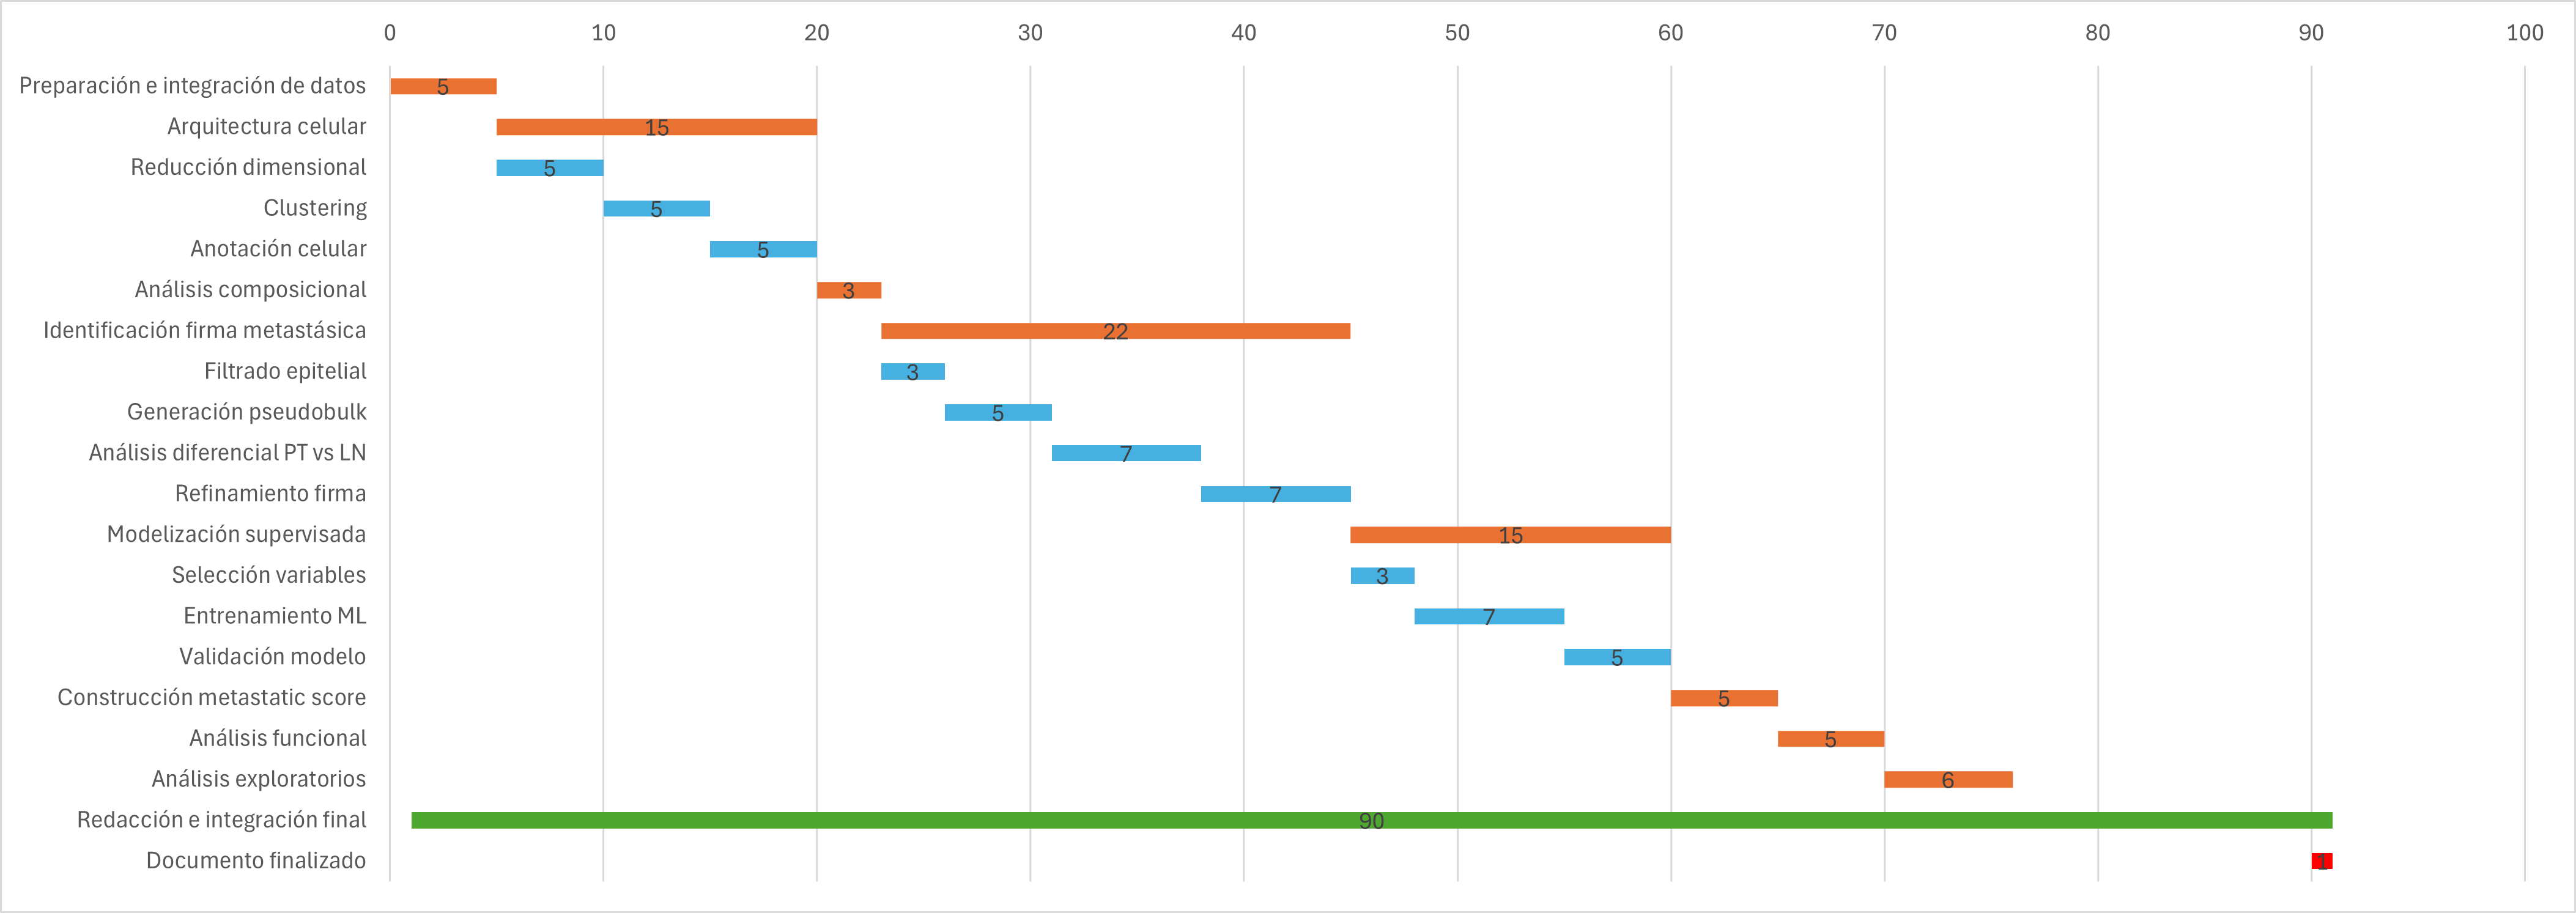
\includegraphics[width=\textwidth]{Gantt.png}
				\caption{Diagrama de Gantt: calendario y distribución temporal de tareas. El color naranja es indicativo de tarea; el color azul, de subtarea; el verde, de tarea transversal; y el rojo, de hito final. El número en el color indica la duración estimada en días.} \label{fig:Gantt}
			\end{figure}
			
		
		\subsection{Hitos}
			\begin{enumerate}
				\item Matriz de expresión validada e integrada con metadatos completos.
				
				\item Mapa celular anotado con identificación de compartimento epitelial tumoral.
				
				\item Evaluación preliminar del papel del microambiente en la progresión.
				
				\item Lista robusta de genes diferencialmente expresados asociados a metástasis.
				
				\item Modelo discriminativo validado e identificación de genes clave.
				
				\item Métrica cuantitativa de activación del programa metastásico.
				
				\item Identificación de procesos biológicos asociados a la firma metastásica.
				
				\item Evaluación contextual de la firma metastásica.
				
				\item Documento completo listo para entrega.
			\end{enumerate}
		
		\subsection{Análisis de riesgos}
		
		Los riesgos analizados se encuentran en la tabla \ref{tab:tabla_riesgos}.
		
		\begin{table}[h!]
			\centering
			\caption{Tabla de análisis de riesgos} \label{tab:tabla_riesgos}
			\resizebox{\textwidth}{!}{
			\begin{tabular}{|p{0.15\textwidth}|p{0.27\textwidth}|p{0.17\textwidth}|p{0.15\textwidth}|p{0.27\textwidth}|}
				\hline
				\textbf{Riesgo} & \textbf{Descripción} & \textbf{Impacto potencial} & \textbf{Probabilidad} & \textbf{Estrategia de mitigación} \\
				\hline
				Alcance excesivo del proyecto & Intentar abordar simultáneamente heterogeneidad celular, firma metastásica, validación clínica fuerte y comparación con normal. & Dispersión de resultados y pérdida de foco & Media & Priorizar los objetivos específicos centrales (firma metastásica PT vs LN) y relegar los análisis exploratorios si el tiempo es limitado. \\
				\hline
				Limitación temporal & El análisis single-cell y ML requiere iteraciones, validación y optimización & Resultados incompletos o poco refinados. & Media & Definir desde el inicio un flujo de análisis cerrado y evitar cambios metodológicos tardíos. \\
				\hline
				Señal biológica insuficiente & Las diferencias transcriptómicas  podrían ser débiles, altamente variables o no reproducibles entre pacientes. & Imposibilidad de definir una firma consistente o modelo predictivo robusto & Media & Ajustar alcance del objetivo. \\
				\hline
				Bajo número de pacientes (N=6) & La unidad biológica independiente es limitada & Sobreinterpre- tación estadística o baja potencia. & Alta & Uso de pseudobulk por paciente, validación leave-one-out y formulación prudente de conclusiones. \\
				\hline
				Bajo número de células normales & Solo 19 células normales disponibles. & Comparaciones Normal vs Tumor estadísticamente débiles & Alta & Plantear análisis con tejido normal como exploratorio y no central. \\
				\hline
				Dependencia entre células (pseudorreplicación) & Tratamiento incorrecto de células como observaciones independientes & Inflación artificial de significación. & Alta & Agregación pseudobulk y análisis a nivel paciente. \\
				\hline
				Heterogeneidad interpaciente elevada & Variabilidad biológica real entre pacientes & Dificultad para identificar firma consistente. & Media & Modelos que controlen efecto paciente y evaluación de estabilidad de genes seleccionados. \\
				\hline
				Sobreajuste en modelos de ML & Dataset de tamaño reducido para clasificación supervisada & Modelos con buen rendimiento aparente pero baja generalización. & Media & Validación cruzada estricta y limitación de complejidad del modelo. \\
				\hline
				Problemas en anotación celular & Errores en identificación de tipos celulares. & Interpretación biológica incorrecta & Media & Uso combinado de métodos automáticos (SingleR) y marcadores conocidos. \\
				\hline
				Resultados biológicamente poco interpretables & Firma sin enriquecimiento funcional claro. & Dificultad en discusión científica & Baja-media & Análisis de enriquecimiento en múltiples bases y contextualización en literatura. \\
				\hline
				Problemas técnicos en integración de archivos TPM & Errores en construcción de matriz de expresión. & Retrasos iniciales & Baja & Validación paso a paso y control de consistencia de datos. \\
				\hline
			\end{tabular}
		}
		\end{table}

	
	\section{Resultados esperados}
	
	Al finalizar el proyecto se espera obtener:
	
	\begin{itemize}
		
		\item Una matriz con datos scRNAseq curada y documentada.
		
		\item Caracterización de la arquitectura celular tumoral.
		
		\item Lista de genes diferencialmente expresados.
		
%		\item Firma transcriptómica metástasica caracterizada.

		\item Conjunto de genes candidatos asociados a diferencias transcriptómicas entre tumor primario y metástasis ganglionar.
		
		\item Resultados de enriquecimiento funcional.
		
		\item Modelo supervisado entrenado y validado.
		
		\item Definición y cálculo de un puntaje metastásico cuantitativo.
		
		\item Un pipeline reproducible para el análisis de single-cell RNAseq.
		
		\item Código documentado y estructurado para reproducibilidad.
		
	\end{itemize}

	
	\section{Bibliografía}
	
	\begin{enumerate}[label={[\arabic*]}]

		\item Sung, H., Ferlay, J., Siegel, R. L., Laversanne, M., Soerjomataram, I., Jemal, A., \& Bray, F. (2021). Global Cancer Statistics 2020: GLOBOCAN Estimates of Incidence and Mortality Worldwide for 36 Cancers in 185 Countries. CA: a cancer journal for clinicians, 71(3), 209–249. \url{https://doi.org/10.3322/caac.21660} \label{bib:globocan}
		
		\item Dagogo-Jack, I., \& Shaw, A. T. (2018). Tumour heterogeneity and resistance to cancer therapies. Nature reviews. Clinical oncology, 15(2), 81–94. \url{https://doi.org/10.1038/nrclinonc.2017.166} \label{bib:tumor_hetereogeneity}
		
		\item Tang, F., Barbacioru, C., Wang, Y. et al. mRNA-Seq whole-transcriptome analysis of a single cell. Nat Methods 6, 377–382 (2009). \url{https://doi.org/10.1038/nmeth.1315} \label{bib:RNA_seq_trad_1}
		
		\item Kolodziejczyk, A. A., Kim, J. K., Svensson, V., Marioni, J. C., \& Teichmann, S. A. (2015). The technology and biology of single-cell RNA sequencing. Molecular Cell, 58(4), 610–620. \url{https://doi.org/10.1016/j.molcel.2015.04.005}. \label{bib:RNA_seq_trad_2}
		
		\item Bian, S., Hou, Y., Zhou, X., Li, X., Yong, J., Wang, Y., Wang, W., Yan, J., Hu, B., Guo, H., Wang, J., Gao, S., Mao, Y., Dong, J., Zhu, P., Xiu, D., Yan, L., Wen, L., Qiao, J., Tang, F., … Fu, W. (2018). Single-cell multiomics sequencing and analyses of human colorectal cancer. Science (New York, N.Y.), 362(6418), 1060–1063. \url{https://doi.org/10.1126/science.aao3791} \label{bib:PAPER}
		
		\item Luecken, M. D., \& Theis, F. J. (2019). Current best practices in single-cell RNA-seq analysis: a tutorial. Molecular systems biology, 15(6), e8746. \url{https://doi.org/10.15252/msb.20188746} \label{bib:tutorial}
	
	
	\end{enumerate}
	
\end{document}